\documentclass{beamer}
\usepackage{tikz,amsmath,hyperref,graphicx,stackrel,animate}
\usetikzlibrary{positioning,shadows,arrows,shapes,calc}
\newcommand{\argmax}{\operatornamewithlimits{argmax}}
\newcommand{\argmin}{\operatornamewithlimits{argmin}}
\mode<presentation>{\usetheme{Frankfurt}}
\AtBeginSection[]
{
  \begin{frame}<beamer>
    \frametitle{Outline}
    \tableofcontents[currentsection,currentsubsection]
  \end{frame}
}
\title{Lecture 5: Fourier Analysis}
\author{Mark Hasegawa-Johnson}
\date{ECE 401: Signal and Image Analysis}
\begin{document}

% Title
\begin{frame}
  \maketitle
\end{frame}

% Title
\begin{frame}
  \tableofcontents
\end{frame}

%%%%%%%%%%%%%%%%%%%%%%%%%%%%%%%%%%%%%%%%%%%%
\section[Review]{Review: Spectrum}
\setcounter{subsection}{1}

\begin{frame}
  \frametitle{Two-sided spectrum}

  The {\bf spectrum} of $x(t)$ is the set of frequencies, and their
  associated phasors,
  \[
  \mbox{Spectrum}\left( x(t) \right) =
  \left\{ (f_{-N},a_{-N}), \ldots, (f_0,a_0), \ldots, (f_N,a_N) \right\}
  \]
  such that
  \[
  x(t) = \sum_{k=-N}^N a_ke^{j2\pi f_kt}
  \]
\end{frame}

\begin{frame}
  \frametitle{Fourier's theorem}

  One reason the spectrum is useful is that {\bf\em any} periodic
  signal can be written as a sum of cosines.  Fourier's theorem says that
  any $x(t)$ that is periodic, i.e.,
  \[
  x(t+T_0) = x(t)
  \]
  can be written as
  \[
  x(t) = \sum_{k=-\infty}^\infty X_k e^{j2\pi k F_0 t}
  \]
  which is a special case of the spectrum for periodic signals:
  $f_k=kF_0$, and $a_k=X_k$, and
  \[
  F_0 = \frac{1}{T_0}
  \]
\end{frame}

\begin{frame}
  \frametitle{Analysis and Synthesis}

  \begin{itemize}
  \item {\bf Fourier Synthesis} is the process of generating the
    signal, $x(t)$, given its spectrum.  Last lecture, you learned
    how to do this, in general.
  \item {\bf Fourier Analysis} is the process of finding the spectrum,
    $X_k$, given the signal $x(t)$.  I'll tell you how to do that today.
  \end{itemize}
\end{frame}

%%%%%%%%%%%%%%%%%%%%%%%%%%%%%%%%%%%%%%%%%%%%
\section[Orthogonality]{Orthogonality}
\setcounter{subsection}{1}

\begin{frame}
  \frametitle{Orthogonality}

  Two functions $f(t)$ and $g(t)$ are said to be {\bf orthogonal}, over
  some period of time $T$, if
  \[
  \int_0^T f(t)g(t) = 0
  \]
\end{frame}

\begin{frame}
  \frametitle{Sine and Cosine are Orthogonal}

  For example, $\sin(2\pi t)$ and $\cos(2\pi t)$ are orthogonal over
  the period $0\le t\le 1$:
  \centerline{\includegraphics[height=2.5in]{exp/orthogonality_cos_sin.png}}
\end{frame}

\begin{frame}
  \frametitle{Sinusoids at Different Frequencies are Orthogonal}

  Similarly, sinusoids at different frequencies are orthogonal over any time
  segment that contains an integer number of periods:
  \centerline{\includegraphics[height=2.5in]{exp/orthogonality_3_4.png}}
\end{frame}

\begin{frame}
  \frametitle{How to use orthogonality}

  Suppose we have a signal that is known to be
  \[
  x(t) = a\cos(2\pi 3t)+b\sin(2\pi 3t)+c\cos(2\pi 4 t)+d\sin(2\pi 4t)+\ldots
  \]
  \ldots but we don't know $a$, $b$, $c$, $d$, etc.  Let's use
  orthogonality to figure out the value of $b$:
  \begin{align*}
    \int_0^1 x(t)\sin(2\pi 3t)dt &= 
    a\int_0^1 \cos(2\pi 3t)\sin(2\pi 3t)dt \\
    &+ b\int_0^1\sin(2\pi 3t)\sin(2\pi 3t)dt\\
    &+ c\int_0^1\cos(2\pi  4t)\sin(2\pi 3t)dt\\
    &+e\int_0^1\sin(2\pi 4t)\sin(2\pi 3t)dt+\ldots
  \end{align*}
\end{frame}

\begin{frame}
  \frametitle{How to use orthogonality}

  \ldots which simplifies to
  \[
  \int_0^1 x(t)\sin(2\pi 3t)dt
  = 0 + b\int_0^1\sin^2(2\pi 3t)dt + 0 + 0 + \ldots
  \]
  The average value of $\sin^2(t)$ is $1/2$, so
  \[
  \int_0^1 x(t)\sin(2\pi 3t)dt = \frac{b}{2}
  \]
  If we {\bf don't} know the value of $b$,
  but we {\bf do} know how to integrate $\int x(t)\sin(2\pi 3t)dt$,
  then we can find the value of $b$ from the formula above.
\end{frame}

\begin{frame}
  \frametitle{How to use orthogonality}
  \centerline{\includegraphics[height=2.5in]{exp/orthogonality_for_spectrum.png}}
\end{frame}

\begin{frame}
  \frametitle{How to use Orthogonality: Fourier Series}

  We still have one problem.  Integrating $\int x(t) \cos(2\pi 4t)dt$
  is hard---lots of ugly integration by parts and so on.  What do we do?
  \begin{enumerate}
  \item {\bf Fourier Series:} Instead of cosine, use complex
    exponential:
    \[
    \int x(t) e^{-j2\pi ft} dt
    \]
    That integral is still hard, but it's always easier than $\int
    x(t) \cos(2\pi 4t)dt$.  It can usually be solved with some
    combination of integration by parts, variable substitution, etc.
  \end{enumerate}
\end{frame}
  
  
%%%%%%%%%%%%%%%%%%%%%%%%%%%%%%%%%%%%%%%%%%%%
\section[Fourier Series]{Fourier Series}
\setcounter{subsection}{1}

\begin{frame}
  \frametitle{Fourier's Theorem}

  Remember Fourier's theorem.  He said that any periodic signal, with
  a period of $T_0$ seconds, can be written
  \[
  x(t) = \sum_{k=-\infty}^\infty X_k e^{j2\pi kt/T_0}
  \]
  What I want to do, now, is to prove that if you know $x(t)$, you can
  find its Fourier series coefficients using the following formula:
  \[
  X_k = \frac{1}{T_0}\int_0^{T_0} x(t)e^{-j2\pi kt/T_0}dt
  \]
\end{frame}

\begin{frame}
  \frametitle{Fourier's Theorem}

  Remember Fourier's theorem.  He said that any periodic signal, with
  a period of $T_0$ seconds, can be written
  \[
  x(t) = \sum_{k=-\infty}^\infty X_k e^{j2\pi kt/T_0}
  \]
  I'm going to find the formula for $X_k$ using the following idea:
  \begin{itemize}
  \item {\bf Orthogonality:} $e^{-j2\pi \ell t/T_0}$ is orthogonal to
    $e^{j2\pi kt/T_0}$ for any $\ell\ne k$.
  \end{itemize}
\end{frame}

\begin{frame}
  \frametitle{Fourier's Theorem and Orthogonality}

  {\bf Orthogonality:} start with $x(t) = \sum_{k=-\infty}^\infty X_k
  e^{j2\pi kt/T_0}$, and multiply both sides by $e^{-j2\pi \ell
    t/T_0}$:
  \[
  x(t)e^{-2\pi\ell t/T_0} = \sum_{k=-\infty}^\infty X_k e^{j2\pi (k-\ell)t/T_0}
  \]
  Now integrate both sides of that equation, over any complete period:
  \[
  \frac{1}{T_0}\int_0^{T_0}x(t)e^{-j2\pi\ell t/T_0}dt =
  \sum_{k=-\infty}^\infty X_k \frac{1}{T_0}\int_0^{T_0} e^{j2\pi (k-\ell)t/T_0}dt
  \]
\end{frame}

\begin{frame}
  \frametitle{Fourier's Theorem and Orthogonality}

  Now think really hard about what's inside that integral sign:
  \begin{align*}
    &\frac{1}{T_0}\int_0^{T_0} e^{j2\pi (k-\ell)t/T_0}dt\\
    &=\frac{1}{T_0}\int_0^{T_0}\cos\left(\frac{2\pi(k-\ell)t}{T_0}\right)dt\\
    &+j\frac{1}{T_0}\int_0^{T_0}\sin\left(\frac{2\pi (k-\ell)t}{T_0}\right)dt
  \end{align*}
  \begin{itemize}
  \item If $k\ne\ell$, then we're integrating a cosine and a sine over
    $k-\ell$ periods.  That integral is always zero.
    \centerline{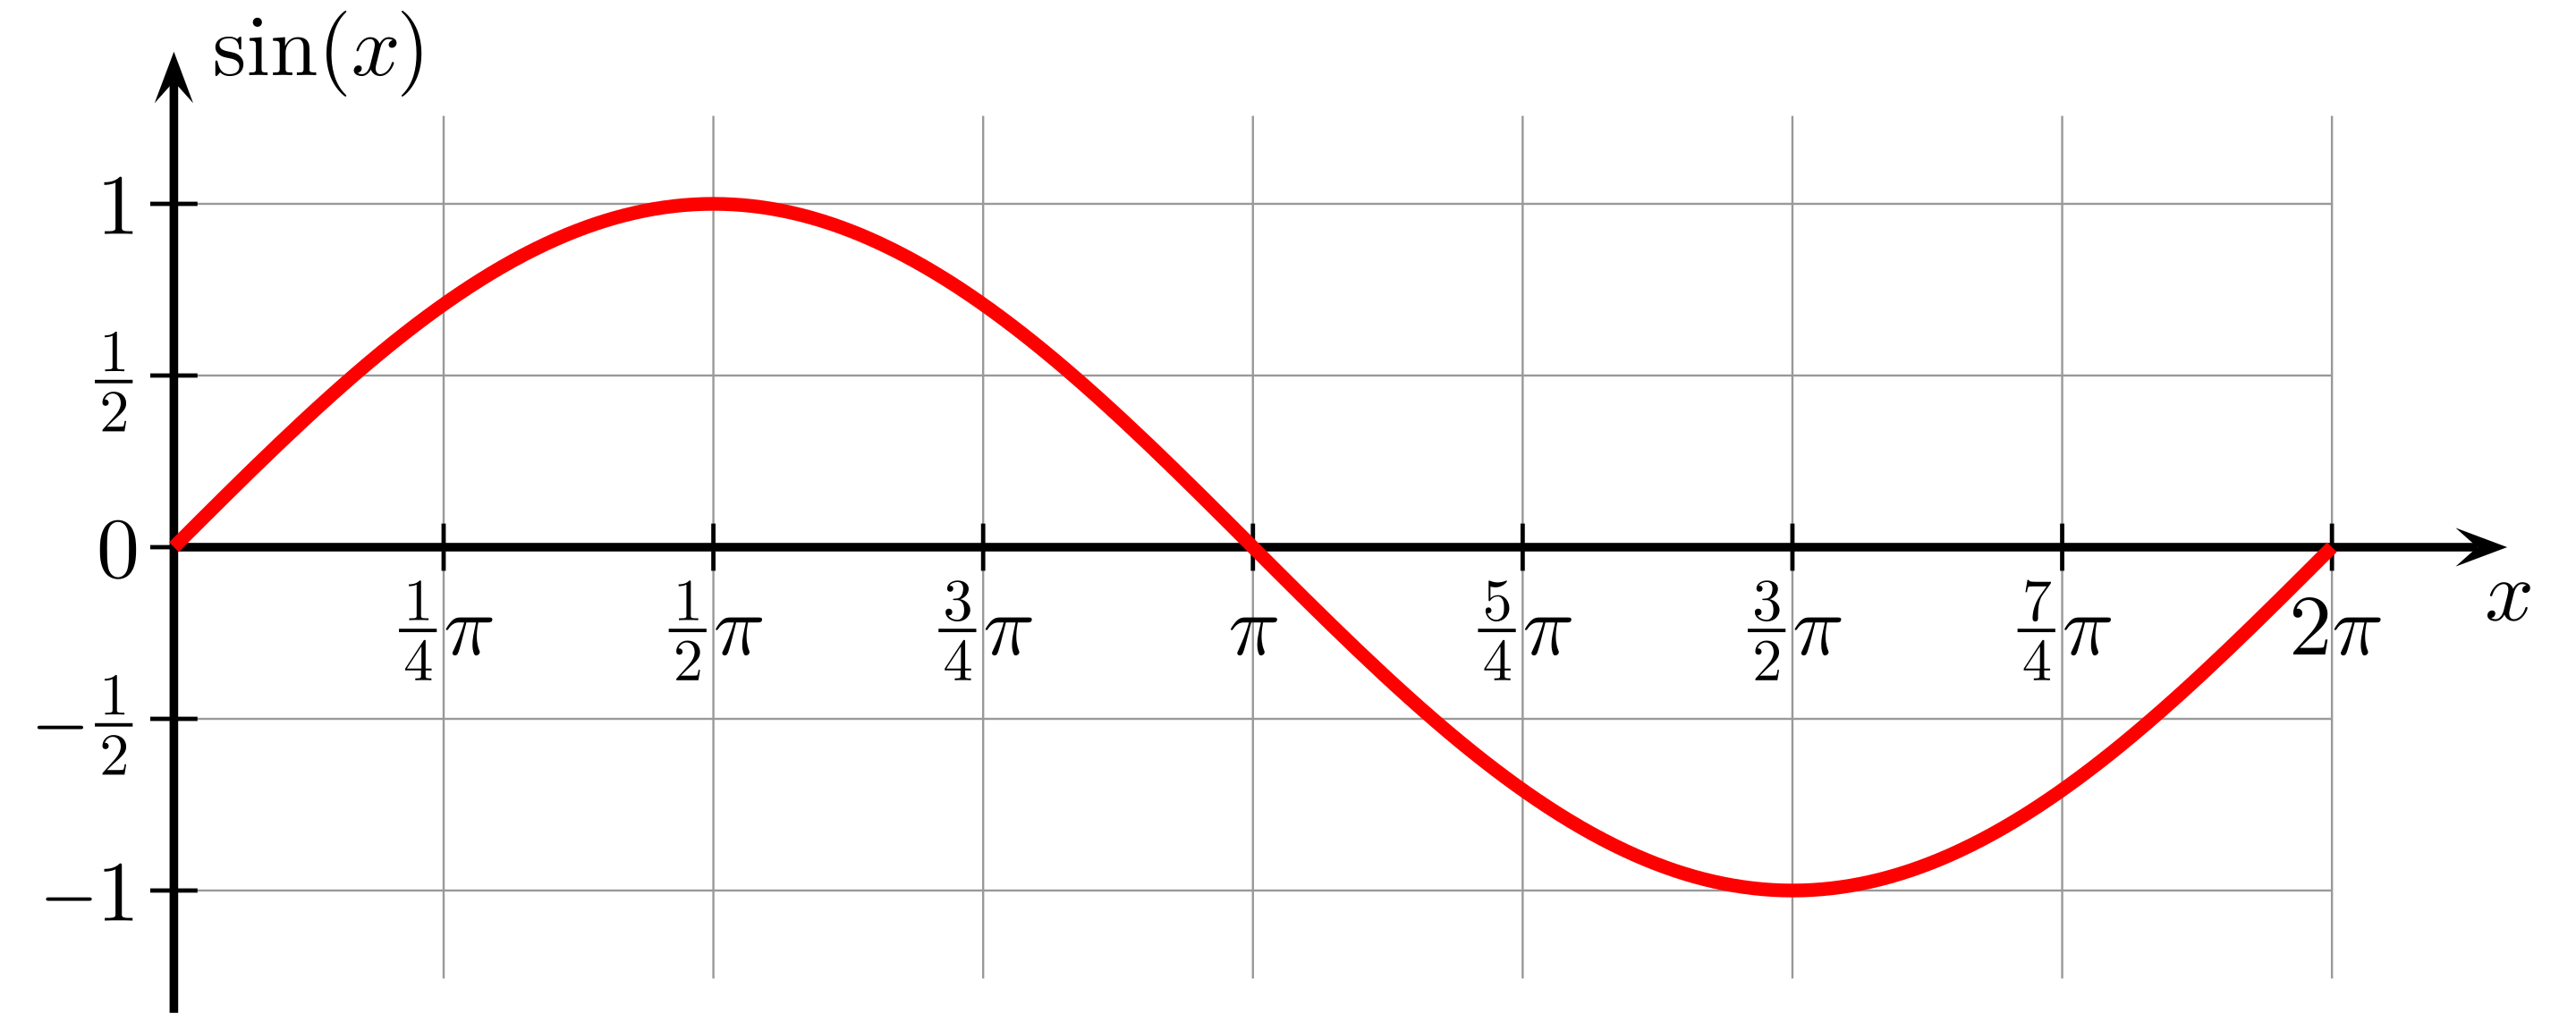
\includegraphics[height=0.25in]{exp/Sine_one_period.png}}
  \item If $k=\ell$, then we're integrating
    \[
    \frac{1}{T_0}\int_0^{T_0}\cos(0)dt+
    j\frac{1}{T_0}\int_0^{T_0}\sin(0)dt = 1
    \]
  \end{itemize}
\end{frame}

\begin{frame}
  \frametitle{Fourier Series: Analysis}

  So, because of orthogonality:
  \begin{align*}
  \frac{1}{T_0}\int_0^{T_0}x(t)e^{-j2\pi\ell t/T_0}dt &=
  \sum_{k=-\infty}^\infty X_k \frac{1}{T_0}\int_0^{T_0} e^{j2\pi (k-\ell)t/T_0}dt\\
  &= \ldots + 0 + 0 + 0 + X_\ell + 0 +0 + 0 + \ldots
  \end{align*}
  
\end{frame}  

\begin{frame}
  \frametitle{Fourier Series}

  \begin{itemize}
  \item {\bf Analysis}  (finding the spectrum, given the waveform):
    \[
    X_k = \frac{1}{T_0}\int_0^{T_0} x(t)e^{-j2\pi kt/T_0}dt
    \]
  \item {\bf Synthesis} (finding the waveform, given the spectrum):
    \[
    x(t) = \sum_{k=-\infty}^\infty X_k e^{j2\pi kt/T_0}
    \]
  \end{itemize}
  
\end{frame}  

%%%%%%%%%%%%%%%%%%%%%%%%%%%%%%%%%%%%%%%%%%%%
\section[Square Wave]{Example: Square Wave}
\setcounter{subsection}{1}

\begin{frame}
  \frametitle{Fourier series: Square wave example}
  \centerline{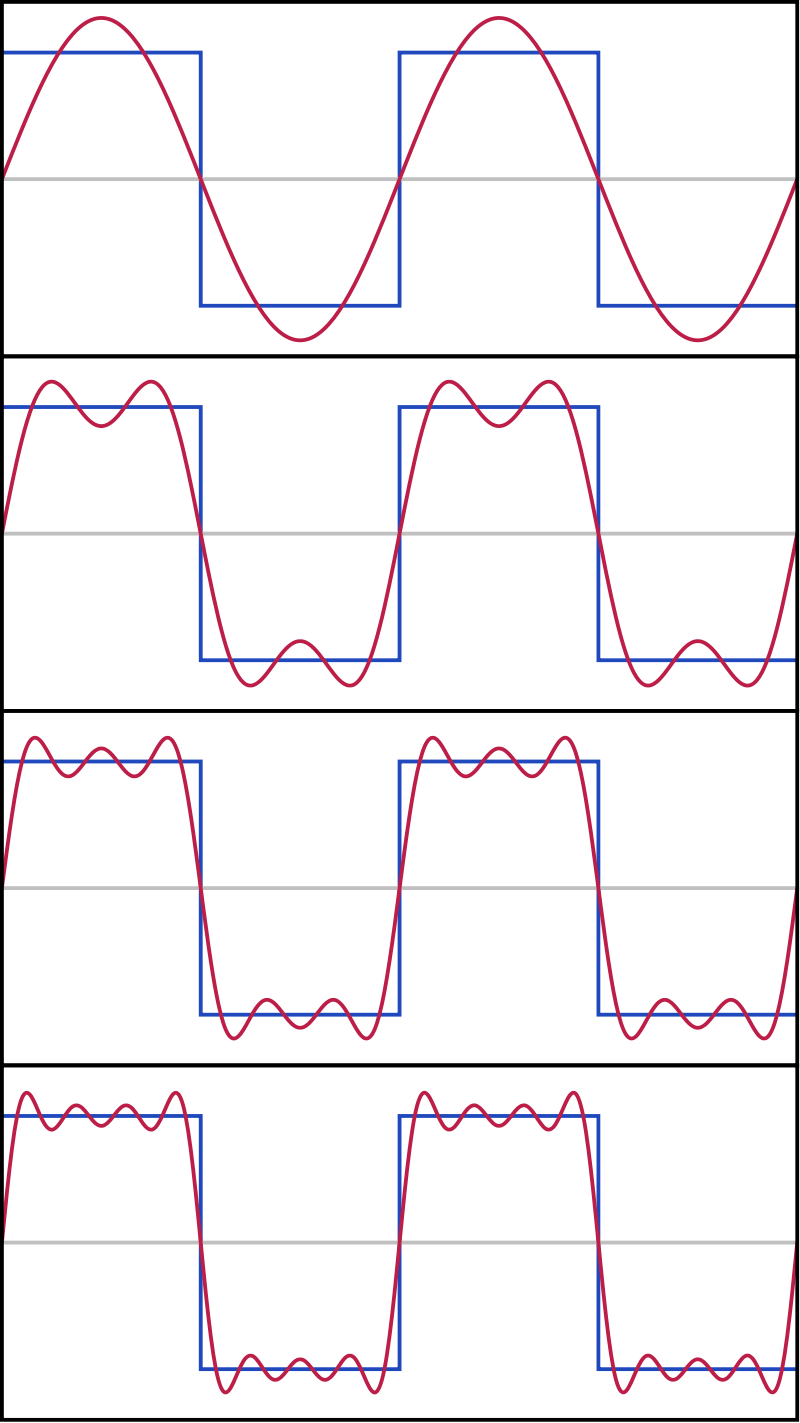
\includegraphics[height=2.5in]{exp/squarewave.png}}
\end{frame}

\begin{frame}
  \frametitle{Square wave example}
  Let's use a square wave with a nonzero DC value, like this one:
  \centerline{\includegraphics[height=2in]{exp/squarewave_alone.png}}
  \[
  x(t) = \left\{\begin{array}{ll}
  1 & -T_0/4 < t < T_0/4 \\
  0 & \mbox{otherwise}
  \end{array}\right.
  \]
\end{frame}

\begin{frame}
  \frametitle{Fourier Series}

  \begin{itemize}
  \item {\bf Analysis}  (finding the spectrum, given the waveform):
    \begin{align*}
    X_k &= \frac{1}{T_0}\int_{-T_0/2}^{T_0/2} x(t)e^{-j2\pi kt/T_0}dt
    \end{align*}
  \end{itemize}
  \centerline{\includegraphics[height=1in]{exp/squarewave_alone.png}}
  
\end{frame}

\begin{frame}
  \frametitle{Fourier Series}

  \begin{itemize}
  \item {\bf Analysis}  (finding the spectrum, given the waveform):
    \begin{align*}
    X_k &= \frac{1}{T_0}\int_{-T_0/2}^{T_0/2} x(t)e^{-j2\pi kt/T_0}dt\\
    &= \frac{1}{T_0}\int_{-T_0/4}^{T_0/4} e^{-j2\pi kt/T_0}dt
    \end{align*}
  \end{itemize}
  \centerline{\includegraphics[height=1in]{exp/squarewave_alone.png}}
  
\end{frame}

\begin{frame}
  \frametitle{Square wave: the $X_0$ term}
    \[
    X_0 = \frac{1}{T_0}\int_{-T_0/4}^{T_0/4} e^{-j2\pi k t/T_0}dt
    \]
    \ldots but if $k=0$, then $e^{-j2\pi kt/T_0}=1$!!!
    \[
    X_0=\frac{1}{T_0}\int_{-T_0/4}^{T_0/4} 1 dt=\frac{1}{2}
    \]
    \centerline{\includegraphics[height=1.5in]{exp/fourierseries0.png}}
\end{frame}

\begin{frame}
  \frametitle{Square wave: the $X_0$ term}
    \[
    X_0 = \frac{1}{2}
    \]
    \centerline{\includegraphics[height=2.5in]{exp/fourierseries0.png}}
\end{frame}

\begin{frame}
  \frametitle{Square wave: the $X_k$ terms, $k\ne 0$}
  \begin{align*}
  X_k &= \frac{1}{T_0}\int_{-T_0/4}^{T_0/4} e^{-j2\pi k t/T_0}dt
  \end{align*}
  \centerline{\includegraphics[height=2.5in]{exp/fourierseries1.png}}
\end{frame}

\begin{frame}
  \frametitle{Square wave: the $X_k$ terms, $k\ne 0$}
  \begin{align*}
    X_k &= \frac{1}{T_0}\int_{-T_0/4}^{T_0/4} e^{-j2\pi k t/T_0}dt\\
    &= \frac{1}{T_0}\left(\frac{1}{-j2\pi k/T_0}\right)\left[e^{-j2\pi k t/T_0}\right]_{-T_0/4}^{T_0/4}\\
    &= \left(\frac{j}{2\pi k}\right)\left[e^{-j2\pi k (T_0/4)/T_0}-e^{-j2\pi k (-T_0/4)/T_0}\right]\\
    &= \left(\frac{j}{2\pi k}\right)\left[e^{-j\pi k/2}-e^{j\pi k/2}\right]\\
    &= \frac{1}{\pi k}\sin\left(\frac{\pi k}{2}\right)\\
    &= \left\{\begin{array}{ll}
    0 & k~\mbox{even}\\
    \pm\frac{1}{\pi k} & k~\mbox{odd}
    \end{array}\right.
  \end{align*}
\end{frame}

\begin{frame}
  \frametitle{Square wave: the $X_1$ terms}
  \[
  X_1 = \frac{1}{\pi}
  \]
  \centerline{\includegraphics[height=2.5in]{exp/fourierseries1.png}}
\end{frame}

\begin{frame}
  \frametitle{Square wave: the $X_2$ term}
    \[
    X_2 = 0
    \]
  \centerline{\includegraphics[height=2.5in]{exp/fourierseries2.png}}
\end{frame}

\begin{frame}
  \frametitle{Square wave: the $X_3$ term}
    \[
    X_3 = -\frac{1}{3\pi}
    \]
  \centerline{\includegraphics[height=2.5in]{exp/fourierseries3.png}}
\end{frame}

\begin{frame}
  \frametitle{Square wave: the $X_5$ term}
    \[
    X_5 = \frac{1}{5\pi}
    \]
  \centerline{\includegraphics[height=2.5in]{exp/fourierseries5.png}}
\end{frame}

\begin{frame}
  \frametitle{Square wave: the whole Fourier series}
    \[
    x(t) = \frac{1}{2} + \frac{1}{\pi}\left(\cos\left(\frac{2\pi t}{T_0}\right)-\frac{1}{3}\cos\left(\frac{6\pi t}{T_0}\right)+\frac{1}{5}\cos\left(\frac{10\pi t}{T_0}\right)-\frac{1}{7}\ldots\right)
    \]
  \centerline{\includegraphics[height=2.5in]{exp/fourierseries5.png}}
\end{frame}

\begin{frame}
  \frametitle{Quiz}

  Try the quiz!  Go to the course webpage, and click on today's date.
\end{frame}

%%%%%%%%%%%%%%%%%%%%%%%%%%%%%%%%%%%%%%%%%%%%
\section[Summary]{Summary}
\setcounter{subsection}{1}

\begin{frame}
  \frametitle{Summary}
  \begin{itemize}
  \item {\bf Analysis}  (finding the spectrum, given the waveform):
    \[
    X_k = \frac{1}{T_0}\int_0^{T_0} x(t)e^{-j2\pi kt/T_0}dt
    \]
  \item {\bf Synthesis}  (finding the waveform, given the spectrum):
    \[
    x(t) = \sum_{k=-\infty}^\infty X_k e^{j2\pi kt/T_0}
    \]
  \end{itemize}
\end{frame}  
        
\end{document}
